% Created by tikzDevice version 0.7.0 on 2014-06-17 19:19:03
% !TEX encoding = UTF-8 Unicode
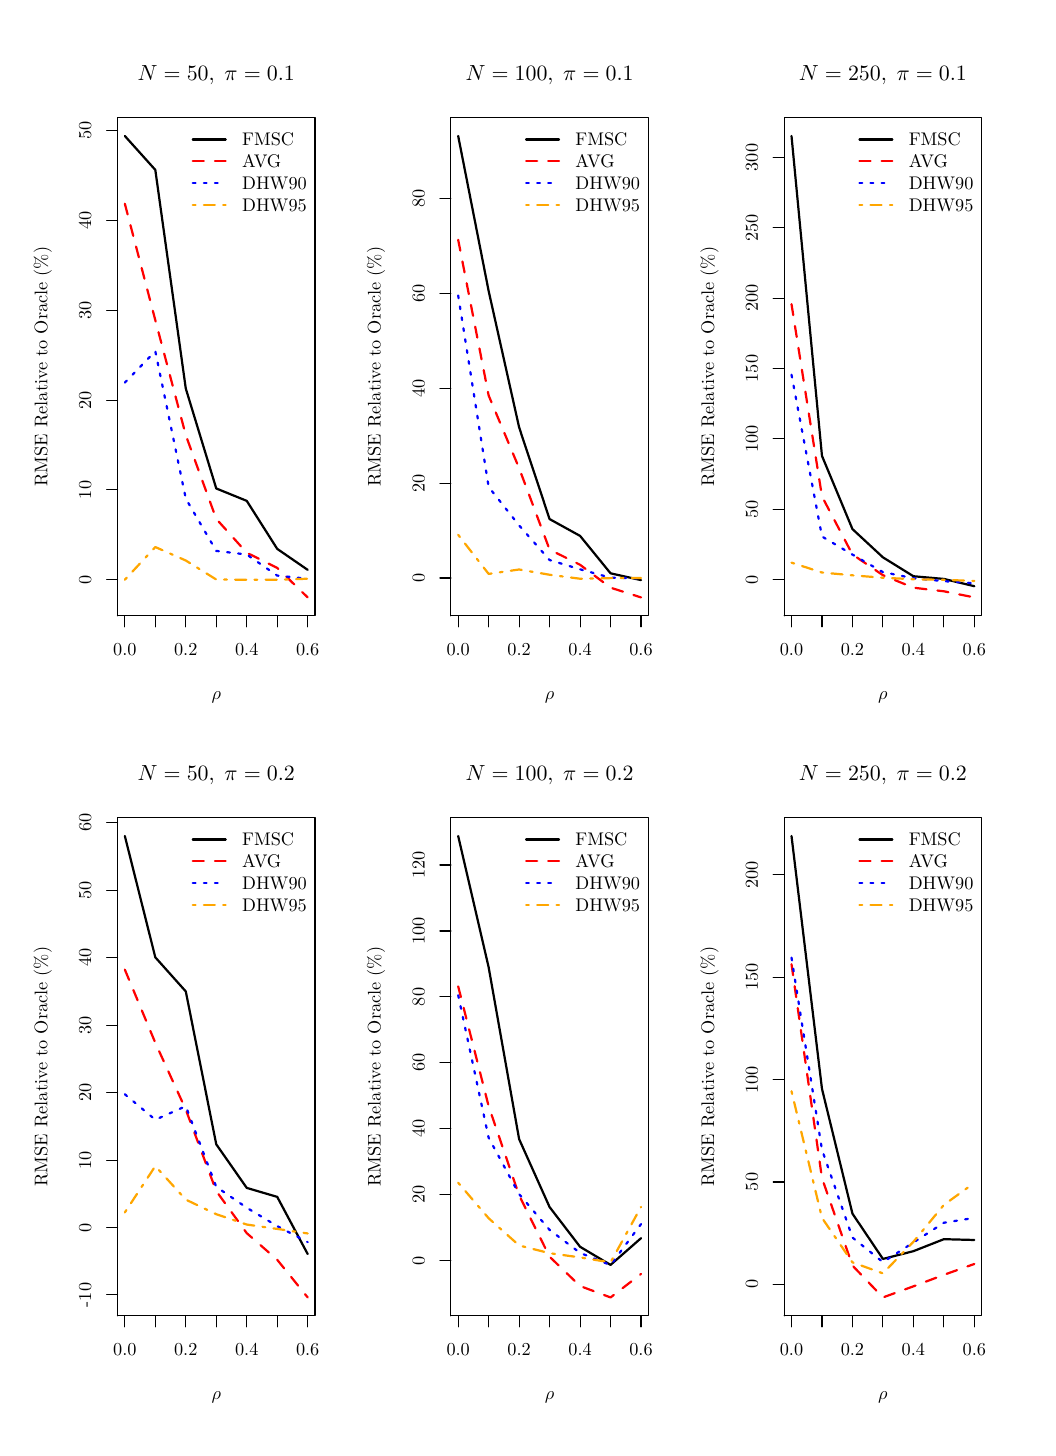
\begin{tikzpicture}[x=1pt,y=1pt]
\definecolor[named]{fillColor}{rgb}{1.00,1.00,1.00}
\path[use as bounding box,fill=fillColor,fill opacity=0.00] (0,0) rectangle (361.35,505.89);
\begin{scope}
\path[clip] ( 32.47,293.34) rectangle (103.82,473.42);
\definecolor[named]{drawColor}{rgb}{0.00,0.00,0.00}

\path[draw=drawColor,line width= 0.8pt,line join=round,line cap=round] ( 35.11,466.75) --
	( 46.12,454.50) --
	( 57.13,375.50) --
	( 68.14,339.38) --
	( 79.16,334.90) --
	( 90.17,317.55) --
	(101.18,309.97);
\end{scope}
\begin{scope}
\path[clip] (  0.00,  0.00) rectangle (361.35,505.89);
\definecolor[named]{drawColor}{rgb}{0.00,0.00,0.00}

\path[draw=drawColor,line width= 0.4pt,line join=round,line cap=round] ( 35.11,293.34) -- (101.18,293.34);

\path[draw=drawColor,line width= 0.4pt,line join=round,line cap=round] ( 35.11,293.34) -- ( 35.11,289.38);

\path[draw=drawColor,line width= 0.4pt,line join=round,line cap=round] ( 46.12,293.34) -- ( 46.12,289.38);

\path[draw=drawColor,line width= 0.4pt,line join=round,line cap=round] ( 57.13,293.34) -- ( 57.13,289.38);

\path[draw=drawColor,line width= 0.4pt,line join=round,line cap=round] ( 68.14,293.34) -- ( 68.14,289.38);

\path[draw=drawColor,line width= 0.4pt,line join=round,line cap=round] ( 79.16,293.34) -- ( 79.16,289.38);

\path[draw=drawColor,line width= 0.4pt,line join=round,line cap=round] ( 90.17,293.34) -- ( 90.17,289.38);

\path[draw=drawColor,line width= 0.4pt,line join=round,line cap=round] (101.18,293.34) -- (101.18,289.38);

\node[text=drawColor,anchor=base,inner sep=0pt, outer sep=0pt, scale=  0.66] at ( 35.11,279.08) {0.0};

\node[text=drawColor,anchor=base,inner sep=0pt, outer sep=0pt, scale=  0.66] at ( 57.13,279.08) {0.2};

\node[text=drawColor,anchor=base,inner sep=0pt, outer sep=0pt, scale=  0.66] at ( 79.16,279.08) {0.4};

\node[text=drawColor,anchor=base,inner sep=0pt, outer sep=0pt, scale=  0.66] at (101.18,279.08) {0.6};

\path[draw=drawColor,line width= 0.4pt,line join=round,line cap=round] ( 32.47,306.40) -- ( 32.47,468.64);

\path[draw=drawColor,line width= 0.4pt,line join=round,line cap=round] ( 32.47,306.40) -- ( 28.51,306.40);

\path[draw=drawColor,line width= 0.4pt,line join=round,line cap=round] ( 32.47,338.85) -- ( 28.51,338.85);

\path[draw=drawColor,line width= 0.4pt,line join=round,line cap=round] ( 32.47,371.30) -- ( 28.51,371.30);

\path[draw=drawColor,line width= 0.4pt,line join=round,line cap=round] ( 32.47,403.74) -- ( 28.51,403.74);

\path[draw=drawColor,line width= 0.4pt,line join=round,line cap=round] ( 32.47,436.19) -- ( 28.51,436.19);

\path[draw=drawColor,line width= 0.4pt,line join=round,line cap=round] ( 32.47,468.64) -- ( 28.51,468.64);

\node[text=drawColor,rotate= 90.00,anchor=base,inner sep=0pt, outer sep=0pt, scale=  0.66] at ( 22.97,306.40) {0};

\node[text=drawColor,rotate= 90.00,anchor=base,inner sep=0pt, outer sep=0pt, scale=  0.66] at ( 22.97,338.85) {10};

\node[text=drawColor,rotate= 90.00,anchor=base,inner sep=0pt, outer sep=0pt, scale=  0.66] at ( 22.97,371.30) {20};

\node[text=drawColor,rotate= 90.00,anchor=base,inner sep=0pt, outer sep=0pt, scale=  0.66] at ( 22.97,403.74) {30};

\node[text=drawColor,rotate= 90.00,anchor=base,inner sep=0pt, outer sep=0pt, scale=  0.66] at ( 22.97,436.19) {40};

\node[text=drawColor,rotate= 90.00,anchor=base,inner sep=0pt, outer sep=0pt, scale=  0.66] at ( 22.97,468.64) {50};

\path[draw=drawColor,line width= 0.4pt,line join=round,line cap=round] ( 32.47,293.34) --
	(103.82,293.34) --
	(103.82,473.42) --
	( 32.47,473.42) --
	( 32.47,293.34);
\end{scope}
\begin{scope}
\path[clip] (  0.00,252.94) rectangle (120.45,505.89);
\definecolor[named]{drawColor}{rgb}{0.00,0.00,0.00}

\node[text=drawColor,anchor=base,inner sep=0pt, outer sep=0pt, scale=  0.79] at ( 68.14,486.92) {\bfseries $N=50, \;\pi=0.1$};

\node[text=drawColor,anchor=base,inner sep=0pt, outer sep=0pt, scale=  0.66] at ( 68.14,263.24) {$\rho$};

\node[text=drawColor,rotate= 90.00,anchor=base,inner sep=0pt, outer sep=0pt, scale=  0.66] at (  7.13,383.38) {RMSE Relative to Oracle (\%)};
\end{scope}
\begin{scope}
\path[clip] ( 32.47,293.34) rectangle (103.82,473.42);
\definecolor[named]{drawColor}{rgb}{1.00,0.00,0.00}

\path[draw=drawColor,line width= 0.8pt,dash pattern=on 4pt off 4pt ,line join=round,line cap=round] ( 35.11,442.27) --
	( 46.12,400.19) --
	( 57.13,358.66) --
	( 68.14,328.39) --
	( 79.16,316.15) --
	( 90.17,310.68) --
	(101.18,300.01);
\definecolor[named]{drawColor}{rgb}{0.00,0.00,1.00}

\path[draw=drawColor,line width= 0.8pt,dash pattern=on 1pt off 3pt ,line join=round,line cap=round] ( 35.11,377.63) --
	( 46.12,388.96) --
	( 57.13,335.73) --
	( 68.14,316.82) --
	( 79.16,315.51) --
	( 90.17,307.90) --
	(101.18,306.75);
\definecolor[named]{drawColor}{rgb}{1.00,0.65,0.00}

\path[draw=drawColor,line width= 0.8pt,dash pattern=on 1pt off 3pt on 4pt off 3pt ,line join=round,line cap=round] ( 35.11,306.40) --
	( 46.12,318.21) --
	( 57.13,313.35) --
	( 68.14,306.47) --
	( 79.16,306.40) --
	( 90.17,306.40) --
	(101.18,306.76);
\definecolor[named]{drawColor}{rgb}{0.00,0.00,0.00}

\path[draw=drawColor,line width= 0.8pt,line join=round,line cap=round] ( 59.66,465.50) -- ( 71.54,465.50);
\definecolor[named]{drawColor}{rgb}{1.00,0.00,0.00}

\path[draw=drawColor,line width= 0.8pt,dash pattern=on 4pt off 4pt ,line join=round,line cap=round] ( 59.66,457.58) -- ( 71.54,457.58);
\definecolor[named]{drawColor}{rgb}{0.00,0.00,1.00}

\path[draw=drawColor,line width= 0.8pt,dash pattern=on 1pt off 3pt ,line join=round,line cap=round] ( 59.66,449.66) -- ( 71.54,449.66);
\definecolor[named]{drawColor}{rgb}{1.00,0.65,0.00}

\path[draw=drawColor,line width= 0.8pt,dash pattern=on 1pt off 3pt on 4pt off 3pt ,line join=round,line cap=round] ( 59.66,441.74) -- ( 71.54,441.74);
\definecolor[named]{drawColor}{rgb}{0.00,0.00,0.00}

\node[text=drawColor,anchor=base west,inner sep=0pt, outer sep=0pt, scale=  0.66] at ( 77.48,463.23) {FMSC};

\node[text=drawColor,anchor=base west,inner sep=0pt, outer sep=0pt, scale=  0.66] at ( 77.48,455.31) {AVG};

\node[text=drawColor,anchor=base west,inner sep=0pt, outer sep=0pt, scale=  0.66] at ( 77.48,447.39) {DHW90};

\node[text=drawColor,anchor=base west,inner sep=0pt, outer sep=0pt, scale=  0.66] at ( 77.48,439.47) {DHW95};
\end{scope}
\begin{scope}
\path[clip] ( 32.47, 40.39) rectangle (103.82,220.47);
\definecolor[named]{drawColor}{rgb}{0.00,0.00,0.00}

\path[draw=drawColor,line width= 0.8pt,line join=round,line cap=round] ( 35.11,213.80) --
	( 46.12,169.96) --
	( 57.13,157.64) --
	( 68.14,102.40) --
	( 79.16, 86.64) --
	( 90.17, 83.40) --
	(101.18, 62.75);
\end{scope}
\begin{scope}
\path[clip] (  0.00,  0.00) rectangle (361.35,505.89);
\definecolor[named]{drawColor}{rgb}{0.00,0.00,0.00}

\path[draw=drawColor,line width= 0.4pt,line join=round,line cap=round] ( 35.11, 40.39) -- (101.18, 40.39);

\path[draw=drawColor,line width= 0.4pt,line join=round,line cap=round] ( 35.11, 40.39) -- ( 35.11, 36.43);

\path[draw=drawColor,line width= 0.4pt,line join=round,line cap=round] ( 46.12, 40.39) -- ( 46.12, 36.43);

\path[draw=drawColor,line width= 0.4pt,line join=round,line cap=round] ( 57.13, 40.39) -- ( 57.13, 36.43);

\path[draw=drawColor,line width= 0.4pt,line join=round,line cap=round] ( 68.14, 40.39) -- ( 68.14, 36.43);

\path[draw=drawColor,line width= 0.4pt,line join=round,line cap=round] ( 79.16, 40.39) -- ( 79.16, 36.43);

\path[draw=drawColor,line width= 0.4pt,line join=round,line cap=round] ( 90.17, 40.39) -- ( 90.17, 36.43);

\path[draw=drawColor,line width= 0.4pt,line join=round,line cap=round] (101.18, 40.39) -- (101.18, 36.43);

\node[text=drawColor,anchor=base,inner sep=0pt, outer sep=0pt, scale=  0.66] at ( 35.11, 26.14) {0.0};

\node[text=drawColor,anchor=base,inner sep=0pt, outer sep=0pt, scale=  0.66] at ( 57.13, 26.14) {0.2};

\node[text=drawColor,anchor=base,inner sep=0pt, outer sep=0pt, scale=  0.66] at ( 79.16, 26.14) {0.4};

\node[text=drawColor,anchor=base,inner sep=0pt, outer sep=0pt, scale=  0.66] at (101.18, 26.14) {0.6};

\path[draw=drawColor,line width= 0.4pt,line join=round,line cap=round] ( 32.47, 47.96) -- ( 32.47,218.55);

\path[draw=drawColor,line width= 0.4pt,line join=round,line cap=round] ( 32.47, 47.96) -- ( 28.51, 47.96);

\path[draw=drawColor,line width= 0.4pt,line join=round,line cap=round] ( 32.47, 72.33) -- ( 28.51, 72.33);

\path[draw=drawColor,line width= 0.4pt,line join=round,line cap=round] ( 32.47, 96.70) -- ( 28.51, 96.70);

\path[draw=drawColor,line width= 0.4pt,line join=round,line cap=round] ( 32.47,121.07) -- ( 28.51,121.07);

\path[draw=drawColor,line width= 0.4pt,line join=round,line cap=round] ( 32.47,145.44) -- ( 28.51,145.44);

\path[draw=drawColor,line width= 0.4pt,line join=round,line cap=round] ( 32.47,169.81) -- ( 28.51,169.81);

\path[draw=drawColor,line width= 0.4pt,line join=round,line cap=round] ( 32.47,194.18) -- ( 28.51,194.18);

\path[draw=drawColor,line width= 0.4pt,line join=round,line cap=round] ( 32.47,218.55) -- ( 28.51,218.55);

\node[text=drawColor,rotate= 90.00,anchor=base,inner sep=0pt, outer sep=0pt, scale=  0.66] at ( 22.97, 47.96) {-10};

\node[text=drawColor,rotate= 90.00,anchor=base,inner sep=0pt, outer sep=0pt, scale=  0.66] at ( 22.97, 72.33) {0};

\node[text=drawColor,rotate= 90.00,anchor=base,inner sep=0pt, outer sep=0pt, scale=  0.66] at ( 22.97, 96.70) {10};

\node[text=drawColor,rotate= 90.00,anchor=base,inner sep=0pt, outer sep=0pt, scale=  0.66] at ( 22.97,121.07) {20};

\node[text=drawColor,rotate= 90.00,anchor=base,inner sep=0pt, outer sep=0pt, scale=  0.66] at ( 22.97,145.44) {30};

\node[text=drawColor,rotate= 90.00,anchor=base,inner sep=0pt, outer sep=0pt, scale=  0.66] at ( 22.97,169.81) {40};

\node[text=drawColor,rotate= 90.00,anchor=base,inner sep=0pt, outer sep=0pt, scale=  0.66] at ( 22.97,194.18) {50};

\node[text=drawColor,rotate= 90.00,anchor=base,inner sep=0pt, outer sep=0pt, scale=  0.66] at ( 22.97,218.55) {60};

\path[draw=drawColor,line width= 0.4pt,line join=round,line cap=round] ( 32.47, 40.39) --
	(103.82, 40.39) --
	(103.82,220.47) --
	( 32.47,220.47) --
	( 32.47, 40.39);
\end{scope}
\begin{scope}
\path[clip] (  0.00,  0.00) rectangle (120.45,252.94);
\definecolor[named]{drawColor}{rgb}{0.00,0.00,0.00}

\node[text=drawColor,anchor=base,inner sep=0pt, outer sep=0pt, scale=  0.79] at ( 68.14,233.98) {\bfseries $N=50, \;\pi=0.2$};

\node[text=drawColor,anchor=base,inner sep=0pt, outer sep=0pt, scale=  0.66] at ( 68.14, 10.30) {$\rho$};

\node[text=drawColor,rotate= 90.00,anchor=base,inner sep=0pt, outer sep=0pt, scale=  0.66] at (  7.13,130.43) {RMSE Relative to Oracle (\%)};
\end{scope}
\begin{scope}
\path[clip] ( 32.47, 40.39) rectangle (103.82,220.47);
\definecolor[named]{drawColor}{rgb}{1.00,0.00,0.00}

\path[draw=drawColor,line width= 0.8pt,dash pattern=on 4pt off 4pt ,line join=round,line cap=round] ( 35.11,165.52) --
	( 46.12,139.07) --
	( 57.13,114.94) --
	( 68.14, 85.51) --
	( 79.16, 70.29) --
	( 90.17, 60.67) --
	(101.18, 47.06);
\definecolor[named]{drawColor}{rgb}{0.00,0.00,1.00}

\path[draw=drawColor,line width= 0.8pt,dash pattern=on 1pt off 3pt ,line join=round,line cap=round] ( 35.11,120.48) --
	( 46.12,111.27) --
	( 57.13,116.17) --
	( 68.14, 87.04) --
	( 79.16, 79.47) --
	( 90.17, 72.84) --
	(101.18, 67.05);
\definecolor[named]{drawColor}{rgb}{1.00,0.65,0.00}

\path[draw=drawColor,line width= 0.8pt,dash pattern=on 1pt off 3pt on 4pt off 3pt ,line join=round,line cap=round] ( 35.11, 77.78) --
	( 46.12, 94.52) --
	( 57.13, 82.41) --
	( 68.14, 77.14) --
	( 79.16, 73.40) --
	( 90.17, 71.82) --
	(101.18, 70.18);
\definecolor[named]{drawColor}{rgb}{0.00,0.00,0.00}

\path[draw=drawColor,line width= 0.8pt,line join=round,line cap=round] ( 59.66,212.55) -- ( 71.54,212.55);
\definecolor[named]{drawColor}{rgb}{1.00,0.00,0.00}

\path[draw=drawColor,line width= 0.8pt,dash pattern=on 4pt off 4pt ,line join=round,line cap=round] ( 59.66,204.63) -- ( 71.54,204.63);
\definecolor[named]{drawColor}{rgb}{0.00,0.00,1.00}

\path[draw=drawColor,line width= 0.8pt,dash pattern=on 1pt off 3pt ,line join=round,line cap=round] ( 59.66,196.71) -- ( 71.54,196.71);
\definecolor[named]{drawColor}{rgb}{1.00,0.65,0.00}

\path[draw=drawColor,line width= 0.8pt,dash pattern=on 1pt off 3pt on 4pt off 3pt ,line join=round,line cap=round] ( 59.66,188.79) -- ( 71.54,188.79);
\definecolor[named]{drawColor}{rgb}{0.00,0.00,0.00}

\node[text=drawColor,anchor=base west,inner sep=0pt, outer sep=0pt, scale=  0.66] at ( 77.48,210.28) {FMSC};

\node[text=drawColor,anchor=base west,inner sep=0pt, outer sep=0pt, scale=  0.66] at ( 77.48,202.36) {AVG};

\node[text=drawColor,anchor=base west,inner sep=0pt, outer sep=0pt, scale=  0.66] at ( 77.48,194.44) {DHW90};

\node[text=drawColor,anchor=base west,inner sep=0pt, outer sep=0pt, scale=  0.66] at ( 77.48,186.52) {DHW95};
\end{scope}
\begin{scope}
\path[clip] (152.92,293.34) rectangle (224.27,473.42);
\definecolor[named]{drawColor}{rgb}{0.00,0.00,0.00}

\path[draw=drawColor,line width= 0.8pt,line join=round,line cap=round] (155.56,466.75) --
	(166.57,410.74) --
	(177.58,361.47) --
	(188.59,328.32) --
	(199.61,322.24) --
	(210.62,308.72) --
	(221.63,306.26);
\end{scope}
\begin{scope}
\path[clip] (  0.00,  0.00) rectangle (361.35,505.89);
\definecolor[named]{drawColor}{rgb}{0.00,0.00,0.00}

\path[draw=drawColor,line width= 0.4pt,line join=round,line cap=round] (155.56,293.34) -- (221.63,293.34);

\path[draw=drawColor,line width= 0.4pt,line join=round,line cap=round] (155.56,293.34) -- (155.56,289.38);

\path[draw=drawColor,line width= 0.4pt,line join=round,line cap=round] (166.57,293.34) -- (166.57,289.38);

\path[draw=drawColor,line width= 0.4pt,line join=round,line cap=round] (177.58,293.34) -- (177.58,289.38);

\path[draw=drawColor,line width= 0.4pt,line join=round,line cap=round] (188.59,293.34) -- (188.59,289.38);

\path[draw=drawColor,line width= 0.4pt,line join=round,line cap=round] (199.61,293.34) -- (199.61,289.38);

\path[draw=drawColor,line width= 0.4pt,line join=round,line cap=round] (210.62,293.34) -- (210.62,289.38);

\path[draw=drawColor,line width= 0.4pt,line join=round,line cap=round] (221.63,293.34) -- (221.63,289.38);

\node[text=drawColor,anchor=base,inner sep=0pt, outer sep=0pt, scale=  0.66] at (155.56,279.08) {0.0};

\node[text=drawColor,anchor=base,inner sep=0pt, outer sep=0pt, scale=  0.66] at (177.58,279.08) {0.2};

\node[text=drawColor,anchor=base,inner sep=0pt, outer sep=0pt, scale=  0.66] at (199.61,279.08) {0.4};

\node[text=drawColor,anchor=base,inner sep=0pt, outer sep=0pt, scale=  0.66] at (221.63,279.08) {0.6};

\path[draw=drawColor,line width= 0.4pt,line join=round,line cap=round] (152.92,307.03) -- (152.92,444.19);

\path[draw=drawColor,line width= 0.4pt,line join=round,line cap=round] (152.92,307.03) -- (148.96,307.03);

\path[draw=drawColor,line width= 0.4pt,line join=round,line cap=round] (152.92,341.32) -- (148.96,341.32);

\path[draw=drawColor,line width= 0.4pt,line join=round,line cap=round] (152.92,375.61) -- (148.96,375.61);

\path[draw=drawColor,line width= 0.4pt,line join=round,line cap=round] (152.92,409.90) -- (148.96,409.90);

\path[draw=drawColor,line width= 0.4pt,line join=round,line cap=round] (152.92,444.19) -- (148.96,444.19);

\node[text=drawColor,rotate= 90.00,anchor=base,inner sep=0pt, outer sep=0pt, scale=  0.66] at (143.42,307.03) {0};

\node[text=drawColor,rotate= 90.00,anchor=base,inner sep=0pt, outer sep=0pt, scale=  0.66] at (143.42,341.32) {20};

\node[text=drawColor,rotate= 90.00,anchor=base,inner sep=0pt, outer sep=0pt, scale=  0.66] at (143.42,375.61) {40};

\node[text=drawColor,rotate= 90.00,anchor=base,inner sep=0pt, outer sep=0pt, scale=  0.66] at (143.42,409.90) {60};

\node[text=drawColor,rotate= 90.00,anchor=base,inner sep=0pt, outer sep=0pt, scale=  0.66] at (143.42,444.19) {80};

\path[draw=drawColor,line width= 0.4pt,line join=round,line cap=round] (152.92,293.34) --
	(224.27,293.34) --
	(224.27,473.42) --
	(152.92,473.42) --
	(152.92,293.34);
\end{scope}
\begin{scope}
\path[clip] (120.45,252.94) rectangle (240.90,505.89);
\definecolor[named]{drawColor}{rgb}{0.00,0.00,0.00}

\node[text=drawColor,anchor=base,inner sep=0pt, outer sep=0pt, scale=  0.79] at (188.59,486.92) {\bfseries $N=100, \;\pi=0.1$};

\node[text=drawColor,anchor=base,inner sep=0pt, outer sep=0pt, scale=  0.66] at (188.59,263.24) {$\rho$};

\node[text=drawColor,rotate= 90.00,anchor=base,inner sep=0pt, outer sep=0pt, scale=  0.66] at (127.58,383.38) {RMSE Relative to Oracle (\%)};
\end{scope}
\begin{scope}
\path[clip] (152.92,293.34) rectangle (224.27,473.42);
\definecolor[named]{drawColor}{rgb}{1.00,0.00,0.00}

\path[draw=drawColor,line width= 0.8pt,dash pattern=on 4pt off 4pt ,line join=round,line cap=round] (155.56,429.24) --
	(166.57,372.98) --
	(177.58,346.72) --
	(188.59,317.30) --
	(199.61,311.80) --
	(210.62,303.53) --
	(221.63,300.01);
\definecolor[named]{drawColor}{rgb}{0.00,0.00,1.00}

\path[draw=drawColor,line width= 0.8pt,dash pattern=on 1pt off 3pt ,line join=round,line cap=round] (155.56,409.11) --
	(166.57,339.94) --
	(177.58,326.02) --
	(188.59,313.52) --
	(199.61,310.17) --
	(210.62,307.13) --
	(221.63,306.91);
\definecolor[named]{drawColor}{rgb}{1.00,0.65,0.00}

\path[draw=drawColor,line width= 0.8pt,dash pattern=on 1pt off 3pt on 4pt off 3pt ,line join=round,line cap=round] (155.56,322.63) --
	(166.57,308.50) --
	(177.58,310.10) --
	(188.59,308.20) --
	(199.61,306.76) --
	(210.62,306.98) --
	(221.63,307.04);
\definecolor[named]{drawColor}{rgb}{0.00,0.00,0.00}

\path[draw=drawColor,line width= 0.8pt,line join=round,line cap=round] (180.11,465.50) -- (191.99,465.50);
\definecolor[named]{drawColor}{rgb}{1.00,0.00,0.00}

\path[draw=drawColor,line width= 0.8pt,dash pattern=on 4pt off 4pt ,line join=round,line cap=round] (180.11,457.58) -- (191.99,457.58);
\definecolor[named]{drawColor}{rgb}{0.00,0.00,1.00}

\path[draw=drawColor,line width= 0.8pt,dash pattern=on 1pt off 3pt ,line join=round,line cap=round] (180.11,449.66) -- (191.99,449.66);
\definecolor[named]{drawColor}{rgb}{1.00,0.65,0.00}

\path[draw=drawColor,line width= 0.8pt,dash pattern=on 1pt off 3pt on 4pt off 3pt ,line join=round,line cap=round] (180.11,441.74) -- (191.99,441.74);
\definecolor[named]{drawColor}{rgb}{0.00,0.00,0.00}

\node[text=drawColor,anchor=base west,inner sep=0pt, outer sep=0pt, scale=  0.66] at (197.93,463.23) {FMSC};

\node[text=drawColor,anchor=base west,inner sep=0pt, outer sep=0pt, scale=  0.66] at (197.93,455.31) {AVG};

\node[text=drawColor,anchor=base west,inner sep=0pt, outer sep=0pt, scale=  0.66] at (197.93,447.39) {DHW90};

\node[text=drawColor,anchor=base west,inner sep=0pt, outer sep=0pt, scale=  0.66] at (197.93,439.47) {DHW95};
\end{scope}
\begin{scope}
\path[clip] (152.92, 40.39) rectangle (224.27,220.47);
\definecolor[named]{drawColor}{rgb}{0.00,0.00,0.00}

\path[draw=drawColor,line width= 0.8pt,line join=round,line cap=round] (155.56,213.80) --
	(166.57,166.37) --
	(177.58,104.28) --
	(188.59, 79.72) --
	(199.61, 65.36) --
	(210.62, 58.82) --
	(221.63, 68.47);
\end{scope}
\begin{scope}
\path[clip] (  0.00,  0.00) rectangle (361.35,505.89);
\definecolor[named]{drawColor}{rgb}{0.00,0.00,0.00}

\path[draw=drawColor,line width= 0.4pt,line join=round,line cap=round] (155.56, 40.39) -- (221.63, 40.39);

\path[draw=drawColor,line width= 0.4pt,line join=round,line cap=round] (155.56, 40.39) -- (155.56, 36.43);

\path[draw=drawColor,line width= 0.4pt,line join=round,line cap=round] (166.57, 40.39) -- (166.57, 36.43);

\path[draw=drawColor,line width= 0.4pt,line join=round,line cap=round] (177.58, 40.39) -- (177.58, 36.43);

\path[draw=drawColor,line width= 0.4pt,line join=round,line cap=round] (188.59, 40.39) -- (188.59, 36.43);

\path[draw=drawColor,line width= 0.4pt,line join=round,line cap=round] (199.61, 40.39) -- (199.61, 36.43);

\path[draw=drawColor,line width= 0.4pt,line join=round,line cap=round] (210.62, 40.39) -- (210.62, 36.43);

\path[draw=drawColor,line width= 0.4pt,line join=round,line cap=round] (221.63, 40.39) -- (221.63, 36.43);

\node[text=drawColor,anchor=base,inner sep=0pt, outer sep=0pt, scale=  0.66] at (155.56, 26.14) {0.0};

\node[text=drawColor,anchor=base,inner sep=0pt, outer sep=0pt, scale=  0.66] at (177.58, 26.14) {0.2};

\node[text=drawColor,anchor=base,inner sep=0pt, outer sep=0pt, scale=  0.66] at (199.61, 26.14) {0.4};

\node[text=drawColor,anchor=base,inner sep=0pt, outer sep=0pt, scale=  0.66] at (221.63, 26.14) {0.6};

\path[draw=drawColor,line width= 0.4pt,line join=round,line cap=round] (152.92, 60.35) -- (152.92,203.30);

\path[draw=drawColor,line width= 0.4pt,line join=round,line cap=round] (152.92, 60.35) -- (148.96, 60.35);

\path[draw=drawColor,line width= 0.4pt,line join=round,line cap=round] (152.92, 84.17) -- (148.96, 84.17);

\path[draw=drawColor,line width= 0.4pt,line join=round,line cap=round] (152.92,108.00) -- (148.96,108.00);

\path[draw=drawColor,line width= 0.4pt,line join=round,line cap=round] (152.92,131.83) -- (148.96,131.83);

\path[draw=drawColor,line width= 0.4pt,line join=round,line cap=round] (152.92,155.65) -- (148.96,155.65);

\path[draw=drawColor,line width= 0.4pt,line join=round,line cap=round] (152.92,179.48) -- (148.96,179.48);

\path[draw=drawColor,line width= 0.4pt,line join=round,line cap=round] (152.92,203.30) -- (148.96,203.30);

\node[text=drawColor,rotate= 90.00,anchor=base,inner sep=0pt, outer sep=0pt, scale=  0.66] at (143.42, 60.35) {0};

\node[text=drawColor,rotate= 90.00,anchor=base,inner sep=0pt, outer sep=0pt, scale=  0.66] at (143.42, 84.17) {20};

\node[text=drawColor,rotate= 90.00,anchor=base,inner sep=0pt, outer sep=0pt, scale=  0.66] at (143.42,108.00) {40};

\node[text=drawColor,rotate= 90.00,anchor=base,inner sep=0pt, outer sep=0pt, scale=  0.66] at (143.42,131.83) {60};

\node[text=drawColor,rotate= 90.00,anchor=base,inner sep=0pt, outer sep=0pt, scale=  0.66] at (143.42,155.65) {80};

\node[text=drawColor,rotate= 90.00,anchor=base,inner sep=0pt, outer sep=0pt, scale=  0.66] at (143.42,179.48) {100};

\node[text=drawColor,rotate= 90.00,anchor=base,inner sep=0pt, outer sep=0pt, scale=  0.66] at (143.42,203.30) {120};

\path[draw=drawColor,line width= 0.4pt,line join=round,line cap=round] (152.92, 40.39) --
	(224.27, 40.39) --
	(224.27,220.47) --
	(152.92,220.47) --
	(152.92, 40.39);
\end{scope}
\begin{scope}
\path[clip] (120.45,  0.00) rectangle (240.90,252.94);
\definecolor[named]{drawColor}{rgb}{0.00,0.00,0.00}

\node[text=drawColor,anchor=base,inner sep=0pt, outer sep=0pt, scale=  0.79] at (188.59,233.98) {\bfseries $N=100, \;\pi=0.2$};

\node[text=drawColor,anchor=base,inner sep=0pt, outer sep=0pt, scale=  0.66] at (188.59, 10.30) {$\rho$};

\node[text=drawColor,rotate= 90.00,anchor=base,inner sep=0pt, outer sep=0pt, scale=  0.66] at (127.58,130.43) {RMSE Relative to Oracle (\%)};
\end{scope}
\begin{scope}
\path[clip] (152.92, 40.39) rectangle (224.27,220.47);
\definecolor[named]{drawColor}{rgb}{1.00,0.00,0.00}

\path[draw=drawColor,line width= 0.8pt,dash pattern=on 4pt off 4pt ,line join=round,line cap=round] (155.56,159.46) --
	(166.57,116.16) --
	(177.58, 83.94) --
	(188.59, 61.77) --
	(199.61, 51.18) --
	(210.62, 47.06) --
	(221.63, 55.54);
\definecolor[named]{drawColor}{rgb}{0.00,0.00,1.00}

\path[draw=drawColor,line width= 0.8pt,dash pattern=on 1pt off 3pt ,line join=round,line cap=round] (155.56,156.25) --
	(166.57,104.76) --
	(177.58, 84.40) --
	(188.59, 71.47) --
	(199.61, 63.16) --
	(210.62, 58.74) --
	(221.63, 73.57);
\definecolor[named]{drawColor}{rgb}{1.00,0.65,0.00}

\path[draw=drawColor,line width= 0.8pt,dash pattern=on 1pt off 3pt on 4pt off 3pt ,line join=round,line cap=round] (155.56, 88.50) --
	(166.57, 75.68) --
	(177.58, 65.84) --
	(188.59, 63.05) --
	(199.61, 61.52) --
	(210.62, 59.72) --
	(221.63, 79.77);
\definecolor[named]{drawColor}{rgb}{0.00,0.00,0.00}

\path[draw=drawColor,line width= 0.8pt,line join=round,line cap=round] (180.11,212.55) -- (191.99,212.55);
\definecolor[named]{drawColor}{rgb}{1.00,0.00,0.00}

\path[draw=drawColor,line width= 0.8pt,dash pattern=on 4pt off 4pt ,line join=round,line cap=round] (180.11,204.63) -- (191.99,204.63);
\definecolor[named]{drawColor}{rgb}{0.00,0.00,1.00}

\path[draw=drawColor,line width= 0.8pt,dash pattern=on 1pt off 3pt ,line join=round,line cap=round] (180.11,196.71) -- (191.99,196.71);
\definecolor[named]{drawColor}{rgb}{1.00,0.65,0.00}

\path[draw=drawColor,line width= 0.8pt,dash pattern=on 1pt off 3pt on 4pt off 3pt ,line join=round,line cap=round] (180.11,188.79) -- (191.99,188.79);
\definecolor[named]{drawColor}{rgb}{0.00,0.00,0.00}

\node[text=drawColor,anchor=base west,inner sep=0pt, outer sep=0pt, scale=  0.66] at (197.93,210.28) {FMSC};

\node[text=drawColor,anchor=base west,inner sep=0pt, outer sep=0pt, scale=  0.66] at (197.93,202.36) {AVG};

\node[text=drawColor,anchor=base west,inner sep=0pt, outer sep=0pt, scale=  0.66] at (197.93,194.44) {DHW90};

\node[text=drawColor,anchor=base west,inner sep=0pt, outer sep=0pt, scale=  0.66] at (197.93,186.52) {DHW95};
\end{scope}
\begin{scope}
\path[clip] (273.37,293.34) rectangle (344.72,473.42);
\definecolor[named]{drawColor}{rgb}{0.00,0.00,0.00}

\path[draw=drawColor,line width= 0.8pt,line join=round,line cap=round] (276.01,466.75) --
	(287.02,351.15) --
	(298.03,324.70) --
	(309.04,314.49) --
	(320.06,307.66) --
	(331.07,306.69) --
	(342.08,304.06);
\end{scope}
\begin{scope}
\path[clip] (  0.00,  0.00) rectangle (361.35,505.89);
\definecolor[named]{drawColor}{rgb}{0.00,0.00,0.00}

\path[draw=drawColor,line width= 0.4pt,line join=round,line cap=round] (276.01,293.34) -- (342.08,293.34);

\path[draw=drawColor,line width= 0.4pt,line join=round,line cap=round] (276.01,293.34) -- (276.01,289.38);

\path[draw=drawColor,line width= 0.4pt,line join=round,line cap=round] (287.02,293.34) -- (287.02,289.38);

\path[draw=drawColor,line width= 0.4pt,line join=round,line cap=round] (298.03,293.34) -- (298.03,289.38);

\path[draw=drawColor,line width= 0.4pt,line join=round,line cap=round] (309.04,293.34) -- (309.04,289.38);

\path[draw=drawColor,line width= 0.4pt,line join=round,line cap=round] (320.06,293.34) -- (320.06,289.38);

\path[draw=drawColor,line width= 0.4pt,line join=round,line cap=round] (331.07,293.34) -- (331.07,289.38);

\path[draw=drawColor,line width= 0.4pt,line join=round,line cap=round] (342.08,293.34) -- (342.08,289.38);

\node[text=drawColor,anchor=base,inner sep=0pt, outer sep=0pt, scale=  0.66] at (276.01,279.08) {0.0};

\node[text=drawColor,anchor=base,inner sep=0pt, outer sep=0pt, scale=  0.66] at (298.03,279.08) {0.2};

\node[text=drawColor,anchor=base,inner sep=0pt, outer sep=0pt, scale=  0.66] at (320.06,279.08) {0.4};

\node[text=drawColor,anchor=base,inner sep=0pt, outer sep=0pt, scale=  0.66] at (342.08,279.08) {0.6};

\path[draw=drawColor,line width= 0.4pt,line join=round,line cap=round] (273.37,306.44) -- (273.37,458.99);

\path[draw=drawColor,line width= 0.4pt,line join=round,line cap=round] (273.37,306.44) -- (269.41,306.44);

\path[draw=drawColor,line width= 0.4pt,line join=round,line cap=round] (273.37,331.87) -- (269.41,331.87);

\path[draw=drawColor,line width= 0.4pt,line join=round,line cap=round] (273.37,357.29) -- (269.41,357.29);

\path[draw=drawColor,line width= 0.4pt,line join=round,line cap=round] (273.37,382.72) -- (269.41,382.72);

\path[draw=drawColor,line width= 0.4pt,line join=round,line cap=round] (273.37,408.14) -- (269.41,408.14);

\path[draw=drawColor,line width= 0.4pt,line join=round,line cap=round] (273.37,433.57) -- (269.41,433.57);

\path[draw=drawColor,line width= 0.4pt,line join=round,line cap=round] (273.37,458.99) -- (269.41,458.99);

\node[text=drawColor,rotate= 90.00,anchor=base,inner sep=0pt, outer sep=0pt, scale=  0.66] at (263.87,306.44) {0};

\node[text=drawColor,rotate= 90.00,anchor=base,inner sep=0pt, outer sep=0pt, scale=  0.66] at (263.87,331.87) {50};

\node[text=drawColor,rotate= 90.00,anchor=base,inner sep=0pt, outer sep=0pt, scale=  0.66] at (263.87,357.29) {100};

\node[text=drawColor,rotate= 90.00,anchor=base,inner sep=0pt, outer sep=0pt, scale=  0.66] at (263.87,382.72) {150};

\node[text=drawColor,rotate= 90.00,anchor=base,inner sep=0pt, outer sep=0pt, scale=  0.66] at (263.87,408.14) {200};

\node[text=drawColor,rotate= 90.00,anchor=base,inner sep=0pt, outer sep=0pt, scale=  0.66] at (263.87,433.57) {250};

\node[text=drawColor,rotate= 90.00,anchor=base,inner sep=0pt, outer sep=0pt, scale=  0.66] at (263.87,458.99) {300};

\path[draw=drawColor,line width= 0.4pt,line join=round,line cap=round] (273.37,293.34) --
	(344.72,293.34) --
	(344.72,473.42) --
	(273.37,473.42) --
	(273.37,293.34);
\end{scope}
\begin{scope}
\path[clip] (240.90,252.94) rectangle (361.35,505.89);
\definecolor[named]{drawColor}{rgb}{0.00,0.00,0.00}

\node[text=drawColor,anchor=base,inner sep=0pt, outer sep=0pt, scale=  0.79] at (309.04,486.92) {\bfseries $N=250, \;\pi=0.1$};

\node[text=drawColor,anchor=base,inner sep=0pt, outer sep=0pt, scale=  0.66] at (309.04,263.24) {$\rho$};

\node[text=drawColor,rotate= 90.00,anchor=base,inner sep=0pt, outer sep=0pt, scale=  0.66] at (248.03,383.38) {RMSE Relative to Oracle (\%)};
\end{scope}
\begin{scope}
\path[clip] (273.37,293.34) rectangle (344.72,473.42);
\definecolor[named]{drawColor}{rgb}{1.00,0.00,0.00}

\path[draw=drawColor,line width= 0.8pt,dash pattern=on 4pt off 4pt ,line join=round,line cap=round] (276.01,405.97) --
	(287.02,336.50) --
	(298.03,315.53) --
	(309.04,308.04) --
	(320.06,303.52) --
	(331.07,302.22) --
	(342.08,300.01);
\definecolor[named]{drawColor}{rgb}{0.00,0.00,1.00}

\path[draw=drawColor,line width= 0.8pt,dash pattern=on 1pt off 3pt ,line join=round,line cap=round] (276.01,380.47) --
	(287.02,322.02) --
	(298.03,315.49) --
	(309.04,309.16) --
	(320.06,306.94) --
	(331.07,305.88) --
	(342.08,305.12);
\definecolor[named]{drawColor}{rgb}{1.00,0.65,0.00}

\path[draw=drawColor,line width= 0.8pt,dash pattern=on 1pt off 3pt on 4pt off 3pt ,line join=round,line cap=round] (276.01,312.58) --
	(287.02,309.01) --
	(298.03,307.99) --
	(309.04,307.12) --
	(320.06,306.58) --
	(331.07,306.36) --
	(342.08,305.96);
\definecolor[named]{drawColor}{rgb}{0.00,0.00,0.00}

\path[draw=drawColor,line width= 0.8pt,line join=round,line cap=round] (300.56,465.50) -- (312.44,465.50);
\definecolor[named]{drawColor}{rgb}{1.00,0.00,0.00}

\path[draw=drawColor,line width= 0.8pt,dash pattern=on 4pt off 4pt ,line join=round,line cap=round] (300.56,457.58) -- (312.44,457.58);
\definecolor[named]{drawColor}{rgb}{0.00,0.00,1.00}

\path[draw=drawColor,line width= 0.8pt,dash pattern=on 1pt off 3pt ,line join=round,line cap=round] (300.56,449.66) -- (312.44,449.66);
\definecolor[named]{drawColor}{rgb}{1.00,0.65,0.00}

\path[draw=drawColor,line width= 0.8pt,dash pattern=on 1pt off 3pt on 4pt off 3pt ,line join=round,line cap=round] (300.56,441.74) -- (312.44,441.74);
\definecolor[named]{drawColor}{rgb}{0.00,0.00,0.00}

\node[text=drawColor,anchor=base west,inner sep=0pt, outer sep=0pt, scale=  0.66] at (318.38,463.23) {FMSC};

\node[text=drawColor,anchor=base west,inner sep=0pt, outer sep=0pt, scale=  0.66] at (318.38,455.31) {AVG};

\node[text=drawColor,anchor=base west,inner sep=0pt, outer sep=0pt, scale=  0.66] at (318.38,447.39) {DHW90};

\node[text=drawColor,anchor=base west,inner sep=0pt, outer sep=0pt, scale=  0.66] at (318.38,439.47) {DHW95};
\end{scope}
\begin{scope}
\path[clip] (273.37, 40.39) rectangle (344.72,220.47);
\definecolor[named]{drawColor}{rgb}{0.00,0.00,0.00}

\path[draw=drawColor,line width= 0.8pt,line join=round,line cap=round] (276.01,213.80) --
	(287.02,122.44) --
	(298.03, 77.34) --
	(309.04, 60.97) --
	(320.06, 63.78) --
	(331.07, 68.11) --
	(342.08, 67.82);
\end{scope}
\begin{scope}
\path[clip] (  0.00,  0.00) rectangle (361.35,505.89);
\definecolor[named]{drawColor}{rgb}{0.00,0.00,0.00}

\path[draw=drawColor,line width= 0.4pt,line join=round,line cap=round] (276.01, 40.39) -- (342.08, 40.39);

\path[draw=drawColor,line width= 0.4pt,line join=round,line cap=round] (276.01, 40.39) -- (276.01, 36.43);

\path[draw=drawColor,line width= 0.4pt,line join=round,line cap=round] (287.02, 40.39) -- (287.02, 36.43);

\path[draw=drawColor,line width= 0.4pt,line join=round,line cap=round] (298.03, 40.39) -- (298.03, 36.43);

\path[draw=drawColor,line width= 0.4pt,line join=round,line cap=round] (309.04, 40.39) -- (309.04, 36.43);

\path[draw=drawColor,line width= 0.4pt,line join=round,line cap=round] (320.06, 40.39) -- (320.06, 36.43);

\path[draw=drawColor,line width= 0.4pt,line join=round,line cap=round] (331.07, 40.39) -- (331.07, 36.43);

\path[draw=drawColor,line width= 0.4pt,line join=round,line cap=round] (342.08, 40.39) -- (342.08, 36.43);

\node[text=drawColor,anchor=base,inner sep=0pt, outer sep=0pt, scale=  0.66] at (276.01, 26.14) {0.0};

\node[text=drawColor,anchor=base,inner sep=0pt, outer sep=0pt, scale=  0.66] at (298.03, 26.14) {0.2};

\node[text=drawColor,anchor=base,inner sep=0pt, outer sep=0pt, scale=  0.66] at (320.06, 26.14) {0.4};

\node[text=drawColor,anchor=base,inner sep=0pt, outer sep=0pt, scale=  0.66] at (342.08, 26.14) {0.6};

\path[draw=drawColor,line width= 0.4pt,line join=round,line cap=round] (273.37, 51.81) -- (273.37,199.73);

\path[draw=drawColor,line width= 0.4pt,line join=round,line cap=round] (273.37, 51.81) -- (269.41, 51.81);

\path[draw=drawColor,line width= 0.4pt,line join=round,line cap=round] (273.37, 88.79) -- (269.41, 88.79);

\path[draw=drawColor,line width= 0.4pt,line join=round,line cap=round] (273.37,125.77) -- (269.41,125.77);

\path[draw=drawColor,line width= 0.4pt,line join=round,line cap=round] (273.37,162.75) -- (269.41,162.75);

\path[draw=drawColor,line width= 0.4pt,line join=round,line cap=round] (273.37,199.73) -- (269.41,199.73);

\node[text=drawColor,rotate= 90.00,anchor=base,inner sep=0pt, outer sep=0pt, scale=  0.66] at (263.87, 51.81) {0};

\node[text=drawColor,rotate= 90.00,anchor=base,inner sep=0pt, outer sep=0pt, scale=  0.66] at (263.87, 88.79) {50};

\node[text=drawColor,rotate= 90.00,anchor=base,inner sep=0pt, outer sep=0pt, scale=  0.66] at (263.87,125.77) {100};

\node[text=drawColor,rotate= 90.00,anchor=base,inner sep=0pt, outer sep=0pt, scale=  0.66] at (263.87,162.75) {150};

\node[text=drawColor,rotate= 90.00,anchor=base,inner sep=0pt, outer sep=0pt, scale=  0.66] at (263.87,199.73) {200};

\path[draw=drawColor,line width= 0.4pt,line join=round,line cap=round] (273.37, 40.39) --
	(344.72, 40.39) --
	(344.72,220.47) --
	(273.37,220.47) --
	(273.37, 40.39);
\end{scope}
\begin{scope}
\path[clip] (240.90,  0.00) rectangle (361.35,252.94);
\definecolor[named]{drawColor}{rgb}{0.00,0.00,0.00}

\node[text=drawColor,anchor=base,inner sep=0pt, outer sep=0pt, scale=  0.79] at (309.04,233.98) {\bfseries $N=250, \;\pi=0.2$};

\node[text=drawColor,anchor=base,inner sep=0pt, outer sep=0pt, scale=  0.66] at (309.04, 10.30) {$\rho$};

\node[text=drawColor,rotate= 90.00,anchor=base,inner sep=0pt, outer sep=0pt, scale=  0.66] at (248.03,130.43) {RMSE Relative to Oracle (\%)};
\end{scope}
\begin{scope}
\path[clip] (273.37, 40.39) rectangle (344.72,220.47);
\definecolor[named]{drawColor}{rgb}{1.00,0.00,0.00}

\path[draw=drawColor,line width= 0.8pt,dash pattern=on 4pt off 4pt ,line join=round,line cap=round] (276.01,167.46) --
	(287.02, 90.16) --
	(298.03, 58.58) --
	(309.04, 47.06) --
	(320.06, 51.07) --
	(331.07, 55.23) --
	(342.08, 59.16);
\definecolor[named]{drawColor}{rgb}{0.00,0.00,1.00}

\path[draw=drawColor,line width= 0.8pt,dash pattern=on 1pt off 3pt ,line join=round,line cap=round] (276.01,169.83) --
	(287.02,100.45) --
	(298.03, 68.71) --
	(309.04, 59.82) --
	(320.06, 66.93) --
	(331.07, 74.05) --
	(342.08, 75.81);
\definecolor[named]{drawColor}{rgb}{1.00,0.65,0.00}

\path[draw=drawColor,line width= 0.8pt,dash pattern=on 1pt off 3pt on 4pt off 3pt ,line join=round,line cap=round] (276.01,121.56) --
	(287.02, 75.81) --
	(298.03, 59.73) --
	(309.04, 55.76) --
	(320.06, 67.16) --
	(331.07, 80.51) --
	(342.08, 88.46);
\definecolor[named]{drawColor}{rgb}{0.00,0.00,0.00}

\path[draw=drawColor,line width= 0.8pt,line join=round,line cap=round] (300.56,212.55) -- (312.44,212.55);
\definecolor[named]{drawColor}{rgb}{1.00,0.00,0.00}

\path[draw=drawColor,line width= 0.8pt,dash pattern=on 4pt off 4pt ,line join=round,line cap=round] (300.56,204.63) -- (312.44,204.63);
\definecolor[named]{drawColor}{rgb}{0.00,0.00,1.00}

\path[draw=drawColor,line width= 0.8pt,dash pattern=on 1pt off 3pt ,line join=round,line cap=round] (300.56,196.71) -- (312.44,196.71);
\definecolor[named]{drawColor}{rgb}{1.00,0.65,0.00}

\path[draw=drawColor,line width= 0.8pt,dash pattern=on 1pt off 3pt on 4pt off 3pt ,line join=round,line cap=round] (300.56,188.79) -- (312.44,188.79);
\definecolor[named]{drawColor}{rgb}{0.00,0.00,0.00}

\node[text=drawColor,anchor=base west,inner sep=0pt, outer sep=0pt, scale=  0.66] at (318.38,210.28) {FMSC};

\node[text=drawColor,anchor=base west,inner sep=0pt, outer sep=0pt, scale=  0.66] at (318.38,202.36) {AVG};

\node[text=drawColor,anchor=base west,inner sep=0pt, outer sep=0pt, scale=  0.66] at (318.38,194.44) {DHW90};

\node[text=drawColor,anchor=base west,inner sep=0pt, outer sep=0pt, scale=  0.66] at (318.38,186.52) {DHW95};
\end{scope}
\end{tikzpicture}
